\begin{maintask}{D}
  \subsection*{課題内容}
  LAN内のiperf3サーバに対し，低速のUDP通信を順方向・逆方向(-R)の双方で行い，スループットとパケットの流れを確認した．

  \subsection*{実験方法}
  \begin{enumerate}
    \item 1つ目のターミナルでキャプチャを開始
      \begin{minted}{zsh}
        tcpdump -i eth1 -s 0 -w day2_D.pcap 'not port 4200'
      \end{minted}

    \item キャプチャ中に，別のターミナルでiperf3を順方向，逆方向の順に実行
      \begin{minted}{zsh}
        (順方向) iperf3 -t 5 -u -b 10k -c 2001:2f8:40:11da::200
        (逆方向) iperf3 -t 5 -R -u -b 10k -c 2001:2f8:40:11da::200
      \end{minted}

    \item キャプチャ側でCtrl-Cを押し，pcapをダウンロードしてWiresharkで開き，フィルタ\texttt{udp.port == 5201}を適用
  \end{enumerate}

  \subsection*{結果}
  tcpdumpの実行結果と，順方向・逆方向のiperf3の実行結果をそれぞれ
  出力\ref{out:tcpdump_d}，
  出力\ref{out:iperf_fwd}，
  出力\ref{out:iperf_rev}
  に示した．

  \begin{termout}[H]
    \caption{tcpdump の実行結果}\label{out:tcpdump_d}
    \begin{minted}{zsh}
    guest@host82:~$ tcpdump -i eth1 -s 0 -w day2_D.pcap 'not port 4200'                                      
    tcpdump: listening on eth1, link-type EN10MB (Ethernet), capture size 262144 bytes                       
    ^C520 packets captured                                                                                   
    522 packets received by filter                                                                           
    0 packets dropped by kernel  
    \end{minted}
  \end{termout}

  \begin{termout}[H]
    \caption{iperf3(順方向) の実行結果}\label{out:iperf_fwd}
    \begin{minted}{zsh}
    guest@host82:~$ iperf3 -t 5 -u -b 10k -c 2001:2f8:40:11da::200                                           
    Connecting to host 2001:2f8:40:11da::200, port 5201                                                      
    [  5] local 2001:2f8:40:11da::182 port 39751 connected to 2001:2f8:40:11da::200 port 5201                
    [ ID] Interval           Transfer     Bitrate         Total Datagrams                                    
    [  5]   0.00-1.00   sec  1.39 KBytes  11.4 Kbits/sec  1                                                  
    [  5]   1.00-2.00   sec  1.39 KBytes  11.4 Kbits/sec  1                                                  
    [  5]   2.00-3.00   sec  1.39 KBytes  11.4 Kbits/sec  1                                                  
    [  5]   3.00-4.00   sec  1.39 KBytes  11.4 Kbits/sec  1                                                  
    [  5]   4.00-5.00   sec  1.39 KBytes  11.4 Kbits/sec  1                                                  
    - - - - - - - - - - - - - - - - - - - - - - - - -                                                        
    [ ID] Interval           Transfer     Bitrate         Jitter    Lost/Total Datagrams                     
    [  5]   0.00-5.00   sec  6.97 KBytes  11.4 Kbits/sec  0.000 ms  0/5 (0%)  sender                         
    [  5]   0.00-5.04   sec  6.97 KBytes  11.3 Kbits/sec  0.003 ms  0/5 (0%)  receiver                       
                                                                                                            
    iperf Done.       
    \end{minted}
  \end{termout}

  \begin{termout}[H]
    \caption{iperf3(逆方向) の実行結果}\label{out:iperf_rev}
    \begin{minted}{zsh}
    guest@host82:~$ iperf3 -t 5 -R -u -b 10k -c 2001:2f8:40:11da::200                                        
    Connecting to host 2001:2f8:40:11da::200, port 5201                                                      
    Reverse mode, remote host 2001:2f8:40:11da::200 is sending                                               
    [  5] local 2001:2f8:40:11da::182 port 37219 connected to 2001:2f8:40:11da::200 port 5201                
    [ ID] Interval           Transfer     Bitrate         Jitter    Lost/Total Datagrams                     
    [  5]   0.00-1.00   sec  1.39 KBytes  11.4 Kbits/sec  2.541 ms  0/1 (0%)                                 
    [  5]   1.00-2.00   sec  1.39 KBytes  11.4 Kbits/sec  4.921 ms  0/1 (0%)                                 
    [  5]   2.00-3.00   sec  1.39 KBytes  11.4 Kbits/sec  4.613 ms  0/1 (0%)                                 
    [  5]   3.00-4.00   sec  1.39 KBytes  11.4 Kbits/sec  4.325 ms  0/1 (0%)                                 
    [  5]   4.00-5.00   sec  1.39 KBytes  11.4 Kbits/sec  4.055 ms  0/1 (0%)                                 
    - - - - - - - - - - - - - - - - - - - - - - - - -                                                        
    [ ID] Interval           Transfer     Bitrate         Jitter    Lost/Total Datagrams                     
    [  5]   0.00-5.04   sec  6.97 KBytes  11.3 Kbits/sec  0.000 ms  0/5 (0%)  sender                         
    [  5]   0.00-5.00   sec  6.97 KBytes  11.4 Kbits/sec  4.055 ms  0/5 (0%)  receiver                       
                                                                                                            
    iperf Done.       
    \end{minted}
  \end{termout}

  \begin{figure}[h]
    \centering
    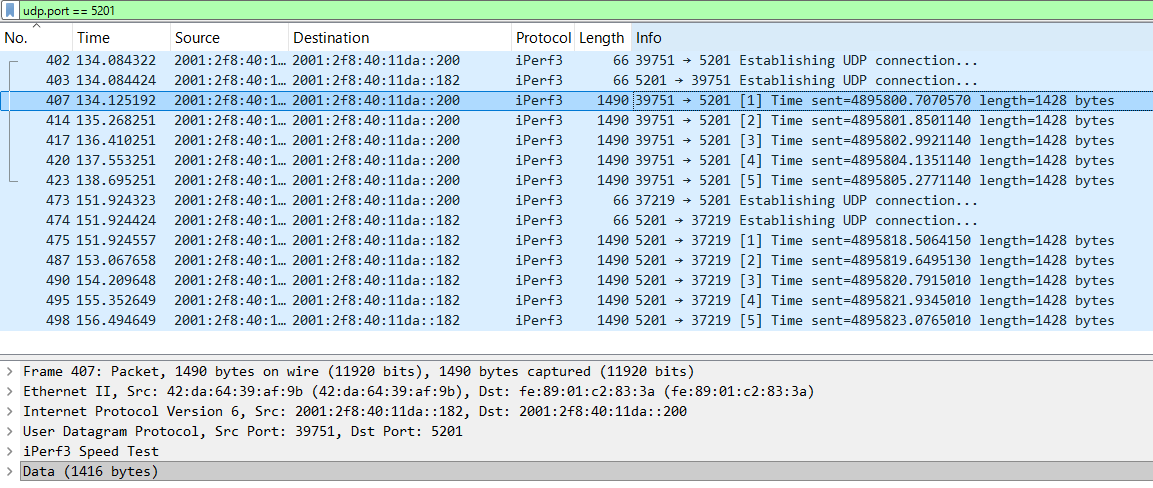
\includegraphics[width=0.98\columnwidth]{fig/wireshark_d_fwd.png}
    \caption{順方向のUDP通信をWiresharkで読み取った結果}
    \label{fig:ws_d_fwd}
  \end{figure}

  \begin{figure}[h]
    \centering
    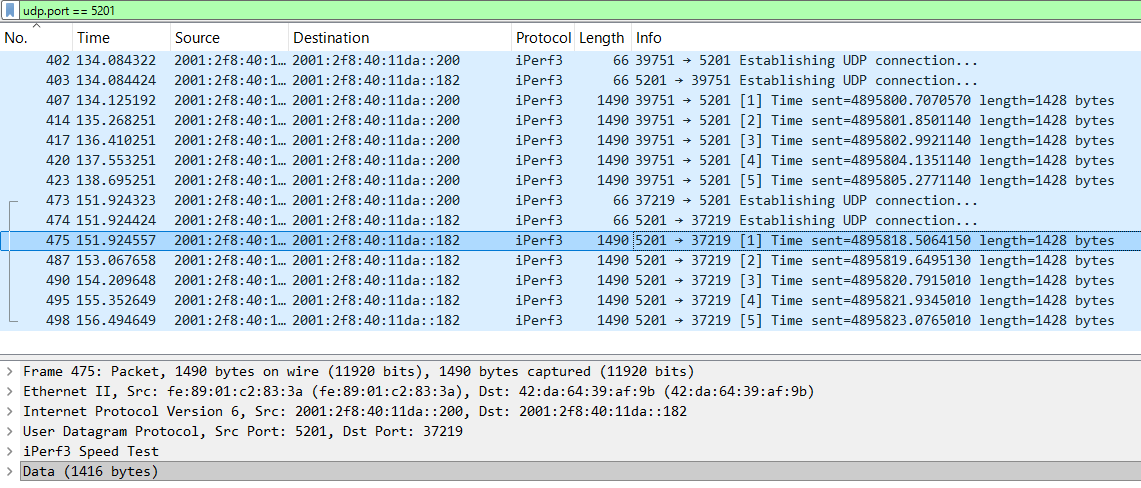
\includegraphics[width=0.98\columnwidth]{fig/wireshark_d_rev.png}
    \caption{逆方向のUDP通信をWiresharkで読み取った結果}
    \label{fig:ws_d_rev}
  \end{figure}

  順方向では，出力\ref{out:iperf_fwd}のとおり，指定した10 kbit/sに対し実測のBitrateは【要記入】であり，【要記入】個のデータグラムを送信して損失は【要記入】であった．図\ref{fig:ws_d_fwd}では，No.【要記入】でクライアント(2001:2f8:40:11da::182)からサーバ(2001:2f8:40:11da::200)のUDP 5201番ポートへ短いデータグラム(【要記入】バイト)が送られ，No.【要記入】でサーバから応答が返っており，これが接続手続きに相当する．その後，No.【要記入】〜【要記入】でデータを含むUDPパケット(ペイロード長【要記入】バイト)が約【要記入】秒間隔で送られている．ペイロード長を$L$バイトとすると，10 kbit/sを保つための送信間隔は$8L/10000$秒であり，$L=$【要記入】のとき【要記入】秒となって観測値と【一致する／しない】．

  逆方向(-R)では，データを送る側がサーバになる．図\ref{fig:ws_d_rev}では，接続手続きののち，サーバ(::200)からクライアント(::182)へデータを含むUDPパケットが送られており，パケットの向きが順方向と入れ替わっている．出力\ref{out:iperf_rev}のBitrateは【要記入】，損失は【要記入】であった．

  なお，フィルタ\texttt{udp.port == 5201}には，iperf3の制御に使われるTCPの接続は含まれない．【要記入：TCP 5201の制御接続を見て気づいたことがあれば】
\end{maintask}
